\documentclass[12pt,fleqn]{article}\usepackage{../../common}
\begin{document}
Ders 6

Bug�n �nceki derste ��rendi�imiz kavramlar� farkl� �ekiller �zerinde
uygulayaca��z. Bu �ekiller i�i bo� �ember / halka, i�i dolu halka ya da
disk, sonsuza giden bir d�zlem (alttaki resim, soldaki �ekil, d�zleme
kenar�ndan bak�l�rsa), ve sonsuza giden iki d�zlem.

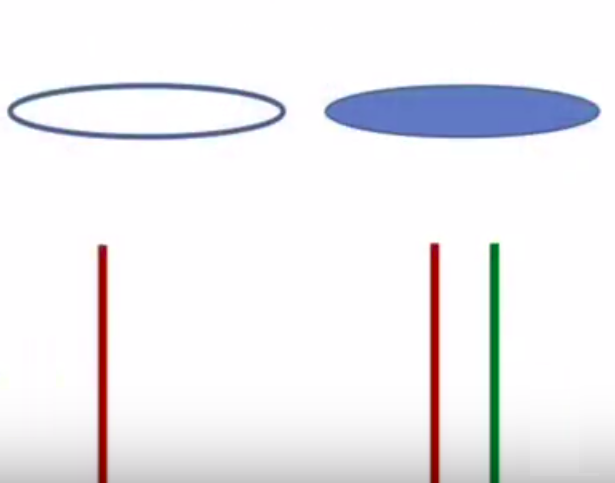
\includegraphics[width=20em]{06_01.png}















\url{https://www.youtube.com/watch?v=WqSa620ln9M}

\end{document}



















